\newpage
\chapter{Experimental results}\label{sec:results}

In this chapter we analyze how Tenmo framework applies to modern multi-layered and hierarchical control plane systems of large-scale service providers (e.g. cloud providers).

\section{Applications}

Tenmo framework has been applied to the following software stack, representative of typical control plane systems. We want to ensure that the selected stack covers the problem domain well, hence we applied the following requirements towards the stack:
%
\begin{itemize}[nosep]
	\item It has to control deployments of a service in a cloud environment.
	\item It has to contain imperative-based processing of user requests.
	\item It has to contain at least 2 distinct intent-based systems in the control flow of a typical request.
	\item It has to be linguistically heterogeneous, i.e. elements of the stack has to be implemented in a diverse set of programming languages.
\end{itemize}

\vskip 1em

The selected stack is the following:
%
\begin{itemize}
	\item Nix is a powerful package manager for Linux and other Unix systems that makes package management reliable and reproducible. It provides atomic upgrades and rollbacks, side-by-side installation of multiple versions of a package, multi-user package management and easy setup of build environments.
	\item KubeNix~\cite{kubenix-xtruder2020Sep} is a Kubernetes resource builder, that uses NixOS module system~\cite[sec. 5]{dolstra2010nixos} for definition of Kubernetes resources and Nix build system for building Kubernetes resources.
	\item Kubectl is a command line tool to interact with a Kuberentes cluster.
	\item Kuberentes is an open-source system for automating deployment, scaling, and management of containerized applications.
    \begin{itemize}
    	\item Kuberentes master is a central server in a Kubernetes cluster, which terminates API calls and ... TODO
    	\item Kubernetes controller
    \end{itemize}
\end{itemize}

We first describe the application of Tenmo to the selected software\footnote{Source code for these integrations is attached to the thesis and is available at \url{https://github.com/gleber/tenmo-thesis}.}, and next we present results of a set of experiments, to show how Tenmo performs in practical scenarios. We analyse both quantifiable measures (e.g. provenance tracking overhead) and subjective measures (e.g. how useful is the provenance data generated during use of the system).

\subsection{Build systems -- Nix}\label{sec:nix-implementation}

We have integrated Tenmo into Nix to show that Tenmo is capable of dealing with build systems, which are a prime example of intent-based actuation systems. As any other declarative build system, it actually is layered on top of a set of imperative building blocks (e.g. executing a compiler or a shell script).

Nix build process (local non-daemon builds only) has been extended to include more comprehensive execution tracing and provenance tracking information as part of the existing JSON logging protocol. Nix language evaluation can be also provenance-tracked, to additionally track provenance of derivation definitions as evaluated from Nix source files. During evaluation instantiation of \texttt{.drv} files is tracked as writes. Process of evaluation of individual \texttt{.nix} file is recorded as executions. Each execution of an individual build process for a derivation records store paths which were consumed and produced (at store path granularity-level).

\begin{figure}[p]
    \centering
    \vspace{-4em}
    \begin{sideways}
\digraph[scale=0.48]{nixSimpleDepsBuild18}{

node [style=filled];
"30447023161345" [id="30447023161345" label="evalu...s/derivation.nix'" shape=rectangle fillcolor=Goldenrod]
"30447023161347" [id="30447023161347" label="evalu...tests/config.nix'" shape=rectangle fillcolor=Goldenrod]
"30447023161346" [id="30447023161346" label="_main.eval" shape=rectangle fillcolor=Goldenrod]
"30447023161350" [id="30447023161350" label="deriv...t-0' being evaled" shape=rectangle fillcolor=Goldenrod]
"30447023161352" [id="30447023161352" label="query...out missing paths" shape=rectangle fillcolor=Goldenrod]
"30447023161356" [id="30447023161356" label="query...out missing paths" shape=rectangle fillcolor=Goldenrod]
"30447023161357" [id="30447023161357" label="build...cies-input-0.drv'" shape=rectangle fillcolor=Goldenrod]
"30447023161358" [id="30447023161358" label="build...ndencies-top.drv'" shape=rectangle fillcolor=Goldenrod]
"30447023161351" [id="30447023161351" label="building 1 paths" shape=rectangle fillcolor=Goldenrod]
"30447023161348" [id="30447023161348" label="prepa... of 1 derivations" shape=rectangle fillcolor=Goldenrod]
"30447023161344" [id="30447023161344" label="_main" shape=rectangle fillcolor=Goldenrod]
"30447023161349" [id="30447023161349" label="deriv...top' being evaled" shape=rectangle fillcolor=Goldenrod]
subgraph "cluster_e:///run/user/1000/nix-test/logging-json/store/40zj9p2w3lkxkpfr3g938vapxp3fmiac-dependencies-input-0.drv" {
id="e:///run/user/1000/nix-test/logging-json/store/40zj9p2w3lkxkpfr3g938vapxp3fmiac-dependencies-input-0.drv";
style=dotted;
fontsize=7;
label="NSO /...r3g938vapxp3fmiac-dependencies-input-0.drv";
"i:///run/user/1000/nix-test/logging-json/store/40zj9p2w3lkxkpfr3g938vapxp3fmiac-dependencies-input-0.drv";
}
subgraph "cluster_e:///run/user/1000/nix-test/logging-json/store/sh0p2kw8ylqzjijdi3cxpl70z857mhbq-dependencies-top.drv" {
id="e:///run/user/1000/nix-test/logging-json/store/sh0p2kw8ylqzjijdi3cxpl70z857mhbq-dependencies-top.drv";
style=dotted;
fontsize=7;
label="NSO /...zjijdi3cxpl70z857mhbq-dependencies-top.drv";
"i:///run/user/1000/nix-test/logging-json/store/sh0p2kw8ylqzjijdi3cxpl70z857mhbq-dependencies-top.drv";
}
subgraph "cluster_e:///run/user/1000/nix-test/logging-json/store/a2k781ggfk1syl2an5y2gx2l8a2yy715-builder-dependencies-input-0.sh" {
id="e:///run/user/1000/nix-test/logging-json/store/a2k781ggfk1syl2an5y2gx2l8a2yy715-builder-dependencies-input-0.sh";
style=dotted;
fontsize=7;
label="NSO /...2l8a2yy715-builder-dependencies-input-0.sh";
"i:///run/user/1000/nix-test/logging-json/store/a2k781ggfk1syl2an5y2gx2l8a2yy715-builder-dependencies-input-0.sh";
}
subgraph "cluster_e:///run/user/1000/nix-test/logging-json/store/wfchbfd39qcy4j1q13fh4mjb0wkjjvdh-dependencies-input-0" {
id="e:///run/user/1000/nix-test/logging-json/store/wfchbfd39qcy4j1q13fh4mjb0wkjjvdh-dependencies-input-0";
style=dotted;
fontsize=7;
label="NSO /...y4j1q13fh4mjb0wkjjvdh-dependencies-input-0";
"i:///run/user/1000/nix-test/logging-json/store/wfchbfd39qcy4j1q13fh4mjb0wkjjvdh-dependencies-input-0";
}
subgraph "cluster_e:///run/user/1000/nix-test/logging-json/store/q6ngyanhbcyjr17yrlbbagagrj2clzxd-simple.deps.builder.sh" {
id="e:///run/user/1000/nix-test/logging-json/store/q6ngyanhbcyjr17yrlbbagagrj2clzxd-simple.deps.builder.sh";
style=dotted;
fontsize=7;
label="NSO /...17yrlbbagagrj2clzxd-simple.deps.builder.sh";
"i:///run/user/1000/nix-test/logging-json/store/q6ngyanhbcyjr17yrlbbagagrj2clzxd-simple.deps.builder.sh";
}
subgraph "cluster_e:///run/user/1000/nix-test/logging-json/store/3hknjp8dvfryb4270bc4fyd1r9jshd9c-dependencies-top" {
id="e:///run/user/1000/nix-test/logging-json/store/3hknjp8dvfryb4270bc4fyd1r9jshd9c-dependencies-top";
style=dotted;
fontsize=7;
label="NSO /...dvfryb4270bc4fyd1r9jshd9c-dependencies-top";
"i:///run/user/1000/nix-test/logging-json/store/3hknjp8dvfryb4270bc4fyd1r9jshd9c-dependencies-top";
}
"i:///run/user/1000/nix-test/logging-json/store/40zj9p2w3lkxkpfr3g938vapxp3fmiac-dependencies-input-0.drv" [id="i:///run/user/1000/nix-test/logging-json/store/40zj9p2w3lkxkpfr3g938vapxp3fmiac-dependencies-input-0.drv" fillcolor=YellowGreen label="NSO /...ncies-input-0.drv" style="dotted, filled" shape=diamond]
"i:///run/user/1000/nix-test/logging-json/store/a2k781ggfk1syl2an5y2gx2l8a2yy715-builder-dependencies-input-0.sh" [id="i:///run/user/1000/nix-test/logging-json/store/a2k781ggfk1syl2an5y2gx2l8a2yy715-builder-dependencies-input-0.sh" fillcolor=YellowGreen label="NSO /...encies-input-0.sh" style="dotted, filled" shape=diamond]
"i:///run/user/1000/nix-test/logging-json/store/sh0p2kw8ylqzjijdi3cxpl70z857mhbq-dependencies-top.drv" [id="i:///run/user/1000/nix-test/logging-json/store/sh0p2kw8ylqzjijdi3cxpl70z857mhbq-dependencies-top.drv" fillcolor=YellowGreen label="NSO /...endencies-top.drv" style="dotted, filled" shape=diamond]
"i:///run/user/1000/nix-test/logging-json/store/q6ngyanhbcyjr17yrlbbagagrj2clzxd-simple.deps.builder.sh" [id="i:///run/user/1000/nix-test/logging-json/store/q6ngyanhbcyjr17yrlbbagagrj2clzxd-simple.deps.builder.sh" fillcolor=YellowGreen label="NSO /...e.deps.builder.sh" style="dotted, filled" shape=diamond]
"i:///run/user/1000/nix-test/logging-json/store/wfchbfd39qcy4j1q13fh4mjb0wkjjvdh-dependencies-input-0" [id="i:///run/user/1000/nix-test/logging-json/store/wfchbfd39qcy4j1q13fh4mjb0wkjjvdh-dependencies-input-0" fillcolor=YellowGreen label="NSO /...endencies-input-0" style="dotted, filled" shape=diamond]
"i:///run/user/1000/nix-test/logging-json/store/3hknjp8dvfryb4270bc4fyd1r9jshd9c-dependencies-top" [id="i:///run/user/1000/nix-test/logging-json/store/3hknjp8dvfryb4270bc4fyd1r9jshd9c-dependencies-top" fillcolor=YellowGreen label="NSO /...-dependencies-top" style="dotted, filled" shape=diamond]
"30447023161344" -> "30447023161345"
"30447023161346" -> "30447023161347"
"30447023161344" -> "30447023161346"
"30447023161349" -> "30447023161350"
"30447023161351" -> "30447023161352"
"30447023161351" -> "30447023161356"
"30447023161351" -> "30447023161357"
"30447023161351" -> "30447023161358"
"30447023161348" -> "30447023161351"
"30447023161344" -> "30447023161348"
"30447023161348" -> "30447023161349"
"30447023161350" -> "i:///run/user/1000/nix-test/logging-json/store/40zj9p2w3lkxkpfr3g938vapxp3fmiac-dependencies-input-0.drv" [style=dashed]
"30447023161349" -> "i:///run/user/1000/nix-test/logging-json/store/sh0p2kw8ylqzjijdi3cxpl70z857mhbq-dependencies-top.drv" [style=dashed]
"i:///run/user/1000/nix-test/logging-json/store/40zj9p2w3lkxkpfr3g938vapxp3fmiac-dependencies-input-0.drv" -> "30447023161357" [style=dashed]
"i:///run/user/1000/nix-test/logging-json/store/a2k781ggfk1syl2an5y2gx2l8a2yy715-builder-dependencies-input-0.sh" -> "30447023161357" [style=dashed]
"30447023161357" -> "i:///run/user/1000/nix-test/logging-json/store/wfchbfd39qcy4j1q13fh4mjb0wkjjvdh-dependencies-input-0" [style=dashed]
"i:///run/user/1000/nix-test/logging-json/store/sh0p2kw8ylqzjijdi3cxpl70z857mhbq-dependencies-top.drv" -> "30447023161358" [style=dashed]
"i:///run/user/1000/nix-test/logging-json/store/q6ngyanhbcyjr17yrlbbagagrj2clzxd-simple.deps.builder.sh" -> "30447023161358" [style=dashed]
"i:///run/user/1000/nix-test/logging-json/store/wfchbfd39qcy4j1q13fh4mjb0wkjjvdh-dependencies-input-0" -> "30447023161358" [style=dashed]
"30447023161358" -> "i:///run/user/1000/nix-test/logging-json/store/3hknjp8dvfryb4270bc4fyd1r9jshd9c-dependencies-top" [style=dashed]


}
\end{sideways}
    \vspace{-2em}
    \caption{Record of a Nix build of two derivations \texttt{top} and \texttt{input0}.} 
    \label{fig:nix-simple-deps-build}
\end{figure}

Nix implementation provides a concept of \texttt{Activity} and \texttt{PushActivity}~\cite{nixloggi85:online}. This allows tracking execution of processes inside of the Nix code base. We made use of this mechanism, since it maps well onto the Tenmo Execution and parent-child executions relationship. Nix's \texttt{cpp}{Activity.result} mechanism was extended and used to register consumed and produced files by executions. Current proof-of-concept Tenmo integration into Nix captures only\footnote{It also captures other existing Nix \texttt{Activity}, but they are not interesting here}:
%
\begin{enumerate}[nosep]
    \item \label{itm:nix-top} Top-level evaluation process as a whole.
    \item Individual \texttt{.nix} file evaluations as children of \cref{itm:nix-top}.
    \item \label{itm:nix-inst} Instantiation of derivations required for the build as children of an artifical execution node representing instantiation process as a whole.
    \item \label{itm:nix-drv-inc} The instantiation from \cref{itm:nix-inst} execution nodes record writes of \texttt{.drv} files as incarnations.
    \item \label{itm:nix-builds} Builds of individual derivations based on \texttt{.drv} files.
    \item Executions capturing builds from \cref{itm:nix-builds} record their reads of \texttt{.drv} incarnations from \cref{itm:nix-drv-inc}, reads of existing Nix store paths (e.g. for a derivation builder scripts), and writes of Nix store paths for their outputs 
\end{enumerate}

This allows us to both trace execution structure of Nix build process\footnote{The visualized graph clearly shows that Nix is a suspending-type of build system~\cite{Mokhov2020}.} and track provenance of Nix store paths.

~\Cref{fig:nix-simple-deps-build}) represents a simple Tenmo record of build execution using a pristine Nix store without any external dependencies (not event \texttt{nixpkgs}). In this build definition \texttt{top} derivation depends on \texttt{input0} derivation. Below we will use names of Nix store paths shortened for brevity by removing \texttt{/nix/store/<hash>} part of it. We could follow this graph and compute direct provenance set of the final build product \texttt{dependencies-top} to be 

\[ \{ \texttt{dependencies-top.drv}, \texttt{dependencies-input-0}, \texttt{simple.deps.builder.sh} \} \]

Its indirect provenance set can be manually computed to be
\begin{equation*}
\begin{split}
\{ & \texttt{dependencies-top.drv}, \texttt{dependencies-input-0}, \texttt{simple.deps.builder.sh}, \\ 
   & \texttt{dependencies-input-0.drv}, \texttt{builder-dependencies-input-0.sh} \} 
\end{split}
\end{equation*}

\bigskip

The same results can be obtained with Tenmo's SQLs (full paths are elided in the output for brevity):
%
\begin{minted}[fontsize=\scriptsize,breaklines]{sql}
tenmo=# select * from provenance_set(
tenmo(#     'i:///.../store/3hknjp8dvfryb4270bc4fyd1r9jshd9c-dependencies-top');
 depth |                                                  obj                                                   
-------+--------------------------------------------------------------------------------
     2 | i:///.../store/sh0p2kw8ylqzjijdi3cxpl70z857mhbq-dependencies-top.drv
     2 | i:///.../store/q6ngyanhbcyjr17yrlbbagagrj2clzxd-simple.deps.builder.sh
     2 | i:///.../store/wfchbfd39qcy4j1q13fh4mjb0wkjjvdh-dependencies-input-0
(3 rows)

tenmo=# select * from provenance_set_indirect(
tenmo(#     'i:///.../store/3hknjp8dvfryb4270bc4fyd1r9jshd9c-dependencies-top');
 depth |                                                       obj                                                       
-------+--------------------------------------------------------------------------------
     2 | i:///.../store/sh0p2kw8ylqzjijdi3cxpl70z857mhbq-dependencies-top.drv
     2 | i:///.../store/q6ngyanhbcyjr17yrlbbagagrj2clzxd-simple.deps.builder.sh
     2 | i:///.../store/wfchbfd39qcy4j1q13fh4mjb0wkjjvdh-dependencies-input-0
     4 | i:///.../store/40zj9p2w3lkxkpfr3g938vapxp3fmiac-dependencies-input-0.drv
     4 | i:///.../store/a2k781ggfk1syl2an5y2gx2l8a2yy715-builder-dependencies-input-0.sh
(5 rows)
\end{minted}

Implementation of \texttt{provenance\_set} and \texttt{provenance\_set\_indirect} these SQL stored procedures is described in \cref{sec:query-implementation}. 

\paragraph*{Future work}

%GP: Czy przenieść to do rozdziału 8 do discussion?

Unstructured line-oriented logs produced by Nix binaries and Nix derivation builds could be attached to the executions as annotations. This would allow to capture a link between build logs and Tenmo execution traces. This mechanism would have a drawback of generating a lot more data to be ingested by the Tenmo pipeline.

We could extend execution of Nix derivation builder with a \texttt{strace}-based tracing mechanism, closely following the CBDG implementation. This would have expanded the results with the ability to capture relationship between Nix derivation build executions and process tree executions happening inside a derivation builder (usually with a shell process acting as a parent, and a compiler as the most prominent child). This gives us execution tracking. File-level tracing of reads and writes would allow to accurately track which files each builder process is using. This gives us operations tracking. Given that Nix model provides a way to map from the file paths to the Nix packages, we can reconstruct accurate entity-subentity provenance graph between files from Nix store and Nix packages. All of the above would allow to have a comprehensive hierarchical tracing and provenance tracking across Nix build process and individual build processes happening inside each Nix derivation build execution.

\subsection{Cluster deployment}

\subsubsection{KubeNix}\label{sec:kubenix}

KubeNix as a Kubernetes resource builder is unique compared to other resource builders, since it combines Nix to build resource definitions and Nixpkgs as a package repository to build deployed containers. KubeNix produces a \texttt{.json} which can be consumed by \texttt{kubectl}. Given that KubeNix is built using Nix, the Tenmo integration with Nix is automatically available for KubeNix operations. An example of a Tenmo trace for a resource builds of \texttt{deployment} with 10 Nginx pod replicas is available in file \texttt{tenmo-thesis/traces/} the thesis code\footnote{The code is also available at \url{https://github.com/gleber/tenmo-thesis} repository.}. It includes a trace for a build with full caches present and just a Nginx configuration being changed. A rebuild operation, which produces no new results.

The trace contains the following number of observed objects:
%
\begin{minted}[fontsize=\scriptsize,breaklines]{sql}
tenmo=> select 'entities', count(entity_id) from entities      
union select 'incarnations', count(incarnation_id) from incarnations
union select 'processes', count(process_id) from processes     
union select 'executions', count('execution_id') from executions
union select 'interactions', count(interaction_id) from interactions
union select 'messages', count(message_id) from messages
union select 'operations', count(operation_id) from operations;
   ?column?   | count 
--------------+-------
 operations   |   958
 processes    |     0
 interactions |     0
 incarnations |   877
 entities     |   877
 messages     |     0
 executions   |  1729
(7 rows)
\end{minted}

It can be seen that the integration does not cover all types of Tenmo objects. Interactions and messages are not crucial for a tool like KubeNix and build system like Nix. One can observe that there is the same number of incarnations as entities, which is a testament to Nix, which immutably stores every Nix store object in the content-addressable manner. That's why we see that very entity is unique and and has a single incarnation associated with it.

When KubeNix is used, the final build result it produced is named \texttt{kubenix-generated.json} and we can observe it's Nix store name recorded by Tenmo:
%
\begin{minted}[fontsize=\scriptsize,breaklines]{sql}
tenmo=> select incarnation_id from incarnations where incarnation_id like '%kubenix-generated.json';
                             incarnation_id                             
------------------------------------------------------------------------
 i:///nix/store/ib4k4scpagnidi7f0imsplfa6zw39vrq-kubenix-generated.json
(1 row)
\end{minted}

It is known that the example deployment resource refers to a a Nginx configuration, hence we can locate an execution which built it:
\begin{minted}[fontsize=\scriptsize,breaklines]{sql}
tenmo=> select incarnation_id from incarnations where incarnation_id like '%nginx-conf.json%';
                           incarnation_id                            
---------------------------------------------------------------------
 i:///nix/store/ryvdjcnb2b1qyzh4fa9nfyp4h1r3063c-nginx-conf.json.drv
(1 row)
\end{minted}

Given these two identifiers it is possible to explore how they relate in the build process:
%
\begin{minted}[fontsize=\scriptsize,breaklines]{sql}
tenmo=> select unnest(path), unnest(verbs) from (select * from get_shortest_path('i:///nix/store/ryvdjcnb2b1qyzh4fa9nfyp4h1r3063c-nginx-conf.json.drv', 'i:///nix/store/ib4k4scpagnidi7f0imsplfa6zw39vrq-kubenix-generated.json', 5) limit 1) t;
                                   unnest                                   |    unnest     
----------------------------------------------------------------------------+---------------
 i:///nix/store/ryvdjcnb2b1qyzh4fa9nfyp4h1r3063c-nginx-conf.json.drv        | written_by
 89154931131069                                                             | child_of
 89154931130415                                                             | writes
 i:///nix/store/mkfqzlb86s6c1vr0llagsm2dsqiz36vp-kubenix-generated.json.drv | read_by
 60967060766724                                                             | writes
 i:///nix/store/ib4k4scpagnidi7f0imsplfa6zw39vrq-kubenix-generated.json     | <destination>
(6 rows)
\end{minted}

Here we search for a single path between these two objects with \texttt{get\_shortest\_path} function with traversal depth limit of 5, and next we unnest the resulting arrays for easier viewing. We can observe that the final generated \texttt{kubenix-generated.json} has been created by an execution with identifier \texttt{60967060766724}, which previously read a \texttt{.drv} file (which is essentially a build recipe). This file was written by an execution \texttt{89154931130415}, which was a child of \texttt{89154931131069}. The latter is the execution, which has instantiated the \texttt{nginx-conf.json.drv} build recipe.

These executions can be looked up to be:
\begin{minted}[fontsize=\scriptsize,breaklines]{sql}
tenmo=> select description, execution_id from executions where execution_id = ANY('{89154931131069,89154931130415,60967060766724}');
                                        description                                        |  execution_id  
-------------------------------------------------------------------------------------------+----------------
 overall building '/nix/store/mkfqzlb86s6c1vr0llagsm2dsqiz36vp-kubenix-generated.json.drv' | 60967060766724
 derivation 'kubenix-generated.json' being evaled                                          | 89154931130415
 derivation 'nginx-conf.json' being evaled                                                 | 89154931131069
(3 rows)
\end{minted}

%% GP: Trace of this contains holes. Nix instrumentation is spotty. I'd need more time to make it more useful to make this section more thorough.

This shows that Tenmo instrumentation of KubeNix -- through Nix -- provides a useful mechanism for exploring the multifaceted build trace. We are able to analyze various types of relationships between executions, incarnations and operations.

\subsubsection{Kubectl}\label{sec:kubectl}

Kubectl is a traditional command line tool, which accepts a definition of the resource as a file (or from standard input), parses it, compares it to the current state of the resource on the Kuberentes cluster, and -- if different -- submits it to the server. Kubectl operates on various kinds of resources, a deployment being our focus. Deployment consists of a replica set, which consists of a number of pods. When Kubectl operates on a deployment, it operates on all of the underlying resources recursively.

We have extended Kubectl to log executions and incarations information about produced resources in the resulting resource description YAML file.\footnote{Every JSON file is a valid YAML file and that's what KubeNix actually produced.}

\begin{figure}[p]
    \centering
    \vspace{-4em}
    \begin{sideways}
\digraph[scale=0.4]{kubectlApply5}{

node [style=filled];
"ex://kubectl-apply-builder-01EJP9RCQ1Y5Q05S9BEP0N17D2" [id="ex://kubectl-apply-builder-01EJP9RCQ1Y5Q05S9BEP0N17D2" label="kubec...resource building" shape=rectangle fillcolor=Goldenrod]
"ex://kubectl-apply-one-01EJP9RDP6M59FTSSRFK74JKSD" [id="ex://kubectl-apply-one-01EJP9RDP6M59FTSSRFK74JKSD" label="kubectl apply one" shape=rectangle fillcolor=Goldenrod]
"ex://kubectl-apply-one-01EJP9RDSYQ8BXNDKD34BPEVV5" [id="ex://kubectl-apply-one-01EJP9RDSYQ8BXNDKD34BPEVV5" label="kubectl apply one" shape=rectangle fillcolor=Goldenrod]
"ex://kubectl-apply-one-01EJP9REENA5M3JB3ECSTCDZ3D" [id="ex://kubectl-apply-one-01EJP9REENA5M3JB3ECSTCDZ3D" label="kubectl apply one" shape=rectangle fillcolor=Goldenrod]
"ex://kubectl-apply-one-01EJP9REJJBGX9ZERMGAEVWEAY" [id="ex://kubectl-apply-one-01EJP9REJJBGX9ZERMGAEVWEAY" label="kubectl apply one" shape=rectangle fillcolor=Goldenrod]
"ex://kubectl-apply-01EJP9RCAVZB25SQGSVJGAV4V9" [id="ex://kubectl-apply-01EJP9RCAVZB25SQGSVJGAV4V9" label="kubectl apply" shape=rectangle fillcolor=Goldenrod]
subgraph "cluster_en://file:///nix/store/va46ws49g08xvyf82fvpzfw7p7bzgjm3-kubenix-generated.json" {
id="en://file:///nix/store/va46ws49g08xvyf82fvpzfw7p7bzgjm3-kubenix-generated.json";
style=dotted;
fontsize=7;
label="file ...yf82fvpzfw7p7bzgjm3-kubenix-generated.json";
"i://file:///nix/store/va46ws49g08xvyf82fvpzfw7p7bzgjm3-kubenix-generated.json?ulid=01EJP9RCQ95JT85A4AJNP67V6C";
}
subgraph "cluster_en://in-memory-/apis/apps/v1/namespaces/default/deployments/nginx" {
id="en://in-memory-/apis/apps/v1/namespaces/default/deployments/nginx";
style=dotted;
fontsize=7;
label="in-me...ps/v1/namespaces/default/deployments/nginx";
"i://in-memory-/apis/apps/v1/namespaces/default/deployments/nginx?ulid=01EJP9RDM2KBXHW0N01QMZSCTZ";
}
subgraph "cluster_en://in-memory-https://192.168.1.1/api/v1/namespaces/default/configmaps/nginx-config" {
id="en://in-memory-https://192.168.1.1/api/v1/namespaces/default/configmaps/nginx-config";
style=dotted;
fontsize=7;
label="in-me...namespaces/default/configmaps/nginx-config";
"i://in-memory-https://192.168.1.1/api/v1/namespaces/default/configmaps/nginx-config?ulid=01EJP9RDMY6BEN4XZBX83ZX0AW";
}
subgraph "cluster_en://in-memory-https://192.168.1.1/api/v1/namespaces/default/configmaps/nginx-static" {
id="en://in-memory-https://192.168.1.1/api/v1/namespaces/default/configmaps/nginx-static";
style=dotted;
fontsize=7;
label="in-me...namespaces/default/configmaps/nginx-static";
"i://in-memory-https://192.168.1.1/api/v1/namespaces/default/configmaps/nginx-static?ulid=01EJP9RDN6VFPTHWG7P6NBGWFC";
}
subgraph "cluster_en://in-memory-https://192.168.1.1/api/v1/namespaces/default/services/nginx" {
id="en://in-memory-https://192.168.1.1/api/v1/namespaces/default/services/nginx";
style=dotted;
fontsize=7;
label="in-me...1/api/v1/namespaces/default/services/nginx";
"i://in-memory-https://192.168.1.1/api/v1/namespaces/default/services/nginx?ulid=01EJP9RDNKD3K51RJACSTS28PA";
}
subgraph "cluster_en:///apis/apps/v1/namespaces/default/deployments/nginx" {
id="en:///apis/apps/v1/namespaces/default/deployments/nginx";
style=dotted;
fontsize=7;
label="resource deployments/nginx";
"i:///apis/apps/v1/namespaces/default/deployments/nginx?ulid=01EJP9RDPT8G67DTE7VN8XX7CX" ->
"i:///apis/apps/v1/namespaces/default/deployments/nginx?ulid=01EJP9RDS7VP68NAQGK4CFW6VH"  [style=invis];
}
subgraph "cluster_en://https://192.168.1.1/api/v1/namespaces/default/configmaps/nginx-config" {
id="en://https://192.168.1.1/api/v1/namespaces/default/configmaps/nginx-config";
style=dotted;
fontsize=7;
label="resource configmaps/nginx-config";
"i://https://192.168.1.1/api/v1/namespaces/default/configmaps/nginx-config?ulid=01EJP9RDTFQFNCK6GYB5DNJY0Z" ->
"i://https://192.168.1.1/api/v1/namespaces/default/configmaps/nginx-config?ulid=01EJP9RE2ZXX51FPC9WT303FQB"  [style=invis];
}
subgraph "cluster_en://https://192.168.1.1/api/v1/namespaces/default/configmaps/nginx-static" {
id="en://https://192.168.1.1/api/v1/namespaces/default/configmaps/nginx-static";
style=dotted;
fontsize=7;
label="resource configmaps/nginx-static";
"i://https://192.168.1.1/api/v1/namespaces/default/configmaps/nginx-static?ulid=01EJP9REFBRQDS6A0JNZF73E80" ->
"i://https://192.168.1.1/api/v1/namespaces/default/configmaps/nginx-static?ulid=01EJP9REHF3W1074H5NWN2MF90"  [style=invis];
}
subgraph "cluster_en://https://192.168.1.1/api/v1/namespaces/default/services/nginx" {
id="en://https://192.168.1.1/api/v1/namespaces/default/services/nginx";
style=dotted;
fontsize=7;
label="resource services/nginx";
"i://https://192.168.1.1/api/v1/namespaces/default/services/nginx?ulid=01EJP9REKAW44WKNW8CC1A80V0" ->
"i://https://192.168.1.1/api/v1/namespaces/default/services/nginx?ulid=01EJP9REP7AB85EW3554GWPR7H" [style=invis];
}
"i://file:///nix/store/va46ws49g08xvyf82fvpzfw7p7bzgjm3-kubenix-generated.json?ulid=01EJP9RCQ95JT85A4AJNP67V6C" [id="i://file:///nix/store/va46ws49g08xvyf82fvpzfw7p7bzgjm3-kubenix-generated.json?ulid=01EJP9RCQ95JT85A4AJNP67V6C" fillcolor=YellowGreen label="file ...ix-generated.json" style="dotted, filled" shape=diamond];
"i://in-memory-/apis/apps/v1/namespaces/default/deployments/nginx?ulid=01EJP9RDM2KBXHW0N01QMZSCTZ" [id="i://in-memory-/apis/apps/v1/namespaces/default/deployments/nginx?ulid=01EJP9RDM2KBXHW0N01QMZSCTZ" fillcolor=YellowGreen label="in-me...deployments/nginx" style="dotted, filled" shape=diamond];
"i:///apis/apps/v1/namespaces/default/deployments/nginx?ulid=01EJP9RDPT8G67DTE7VN8XX7CX" [id="i:///apis/apps/v1/namespaces/default/deployments/nginx?ulid=01EJP9RDPT8G67DTE7VN8XX7CX" fillcolor=YellowGreen label="resou...deployments/nginx" style="dotted, filled" shape=diamond];
"i:///apis/apps/v1/namespaces/default/deployments/nginx?ulid=01EJP9RDS7VP68NAQGK4CFW6VH" [id="i:///apis/apps/v1/namespaces/default/deployments/nginx?ulid=01EJP9RDS7VP68NAQGK4CFW6VH" fillcolor=YellowGreen label="resou...deployments/nginx" style="dotted, filled" shape=diamond];
"i://in-memory-https://192.168.1.1/api/v1/namespaces/default/configmaps/nginx-config?ulid=01EJP9RDMY6BEN4XZBX83ZX0AW" [id="i://in-memory-https://192.168.1.1/api/v1/namespaces/default/configmaps/nginx-config?ulid=01EJP9RDMY6BEN4XZBX83ZX0AW" fillcolor=YellowGreen label="in-me...maps/nginx-config" style="dotted, filled" shape=diamond];
"i://https://192.168.1.1/api/v1/namespaces/default/configmaps/nginx-config?ulid=01EJP9RDTFQFNCK6GYB5DNJY0Z" [id="i://https://192.168.1.1/api/v1/namespaces/default/configmaps/nginx-config?ulid=01EJP9RDTFQFNCK6GYB5DNJY0Z" fillcolor=YellowGreen label="resou...maps/nginx-config" style="dotted, filled" shape=diamond];
"i://https://192.168.1.1/api/v1/namespaces/default/configmaps/nginx-config?ulid=01EJP9RE2ZXX51FPC9WT303FQB" [id="i://https://192.168.1.1/api/v1/namespaces/default/configmaps/nginx-config?ulid=01EJP9RE2ZXX51FPC9WT303FQB" fillcolor=YellowGreen label="resou...maps/nginx-config" style="dotted, filled" shape=diamond];
"i://in-memory-https://192.168.1.1/api/v1/namespaces/default/configmaps/nginx-static?ulid=01EJP9RDN6VFPTHWG7P6NBGWFC" [id="i://in-memory-https://192.168.1.1/api/v1/namespaces/default/configmaps/nginx-static?ulid=01EJP9RDN6VFPTHWG7P6NBGWFC" fillcolor=YellowGreen label="in-me...maps/nginx-static" style="dotted, filled" shape=diamond];
"i://https://192.168.1.1/api/v1/namespaces/default/configmaps/nginx-static?ulid=01EJP9REFBRQDS6A0JNZF73E80" [id="i://https://192.168.1.1/api/v1/namespaces/default/configmaps/nginx-static?ulid=01EJP9REFBRQDS6A0JNZF73E80" fillcolor=YellowGreen label="resou...maps/nginx-static" style="dotted, filled" shape=diamond];
"i://https://192.168.1.1/api/v1/namespaces/default/configmaps/nginx-static?ulid=01EJP9REHF3W1074H5NWN2MF90" [id="i://https://192.168.1.1/api/v1/namespaces/default/configmaps/nginx-static?ulid=01EJP9REHF3W1074H5NWN2MF90" fillcolor=YellowGreen label="resou...maps/nginx-static" style="dotted, filled" shape=diamond];
"i://in-memory-https://192.168.1.1/api/v1/namespaces/default/services/nginx?ulid=01EJP9RDNKD3K51RJACSTS28PA" [id="i://in-memory-https://192.168.1.1/api/v1/namespaces/default/services/nginx?ulid=01EJP9RDNKD3K51RJACSTS28PA" fillcolor=YellowGreen label="in-me...lt/services/nginx" style="dotted, filled" shape=diamond];
"i://https://192.168.1.1/api/v1/namespaces/default/services/nginx?ulid=01EJP9REKAW44WKNW8CC1A80V0" [id="i://https://192.168.1.1/api/v1/namespaces/default/services/nginx?ulid=01EJP9REKAW44WKNW8CC1A80V0" fillcolor=YellowGreen label="resource services/nginx" style="dotted, filled" shape=diamond];
"i://https://192.168.1.1/api/v1/namespaces/default/services/nginx?ulid=01EJP9REP7AB85EW3554GWPR7H" [id="i://https://192.168.1.1/api/v1/namespaces/default/services/nginx?ulid=01EJP9REP7AB85EW3554GWPR7H" fillcolor=YellowGreen label="resource services/nginx" style="dotted, filled" shape=diamond];
"ex://kubectl-apply-01EJP9RCAVZB25SQGSVJGAV4V9" -> "ex://kubectl-apply-builder-01EJP9RCQ1Y5Q05S9BEP0N17D2" [weight=25];
"ex://kubectl-apply-01EJP9RCAVZB25SQGSVJGAV4V9" -> "ex://kubectl-apply-one-01EJP9RDP6M59FTSSRFK74JKSD" [weight=25];
"ex://kubectl-apply-01EJP9RCAVZB25SQGSVJGAV4V9" -> "ex://kubectl-apply-one-01EJP9RDSYQ8BXNDKD34BPEVV5" [weight=25];
"ex://kubectl-apply-01EJP9RCAVZB25SQGSVJGAV4V9" -> "ex://kubectl-apply-one-01EJP9REENA5M3JB3ECSTCDZ3D" [weight=25];
"ex://kubectl-apply-01EJP9RCAVZB25SQGSVJGAV4V9" -> "ex://kubectl-apply-one-01EJP9REJJBGX9ZERMGAEVWEAY" [weight=25];
"i://file:///nix/store/va46ws49g08xvyf82fvpzfw7p7bzgjm3-kubenix-generated.json?ulid=01EJP9RCQ95JT85A4AJNP67V6C" -> "ex://kubectl-apply-builder-01EJP9RCQ1Y5Q05S9BEP0N17D2" [style=dashed weight=10];
"ex://kubectl-apply-builder-01EJP9RCQ1Y5Q05S9BEP0N17D2" -> "i://in-memory-/apis/apps/v1/namespaces/default/deployments/nginx?ulid=01EJP9RDM2KBXHW0N01QMZSCTZ" [style=dashed weight=15];
"ex://kubectl-apply-builder-01EJP9RCQ1Y5Q05S9BEP0N17D2" -> "i://in-memory-https://192.168.1.1/api/v1/namespaces/default/configmaps/nginx-config?ulid=01EJP9RDMY6BEN4XZBX83ZX0AW" [style=dashed weight=15];
"ex://kubectl-apply-builder-01EJP9RCQ1Y5Q05S9BEP0N17D2" -> "i://in-memory-https://192.168.1.1/api/v1/namespaces/default/configmaps/nginx-static?ulid=01EJP9RDN6VFPTHWG7P6NBGWFC" [style=dashed weight=15];
"ex://kubectl-apply-builder-01EJP9RCQ1Y5Q05S9BEP0N17D2" -> "i://in-memory-https://192.168.1.1/api/v1/namespaces/default/services/nginx?ulid=01EJP9RDNKD3K51RJACSTS28PA" [style=dashed weight=15];
"i://in-memory-/apis/apps/v1/namespaces/default/deployments/nginx?ulid=01EJP9RDM2KBXHW0N01QMZSCTZ" -> "ex://kubectl-apply-one-01EJP9RDP6M59FTSSRFK74JKSD" [style=dashed weight=10];
"i:///apis/apps/v1/namespaces/default/deployments/nginx?ulid=01EJP9RDPT8G67DTE7VN8XX7CX" -> "ex://kubectl-apply-one-01EJP9RDP6M59FTSSRFK74JKSD" [style=dashed weight=10];
"ex://kubectl-apply-one-01EJP9RDP6M59FTSSRFK74JKSD" -> "i:///apis/apps/v1/namespaces/default/deployments/nginx?ulid=01EJP9RDS7VP68NAQGK4CFW6VH" [style=dashed weight=15];
"i://in-memory-https://192.168.1.1/api/v1/namespaces/default/configmaps/nginx-config?ulid=01EJP9RDMY6BEN4XZBX83ZX0AW" -> "ex://kubectl-apply-one-01EJP9RDSYQ8BXNDKD34BPEVV5" [style=dashed weight=10];
"i://https://192.168.1.1/api/v1/namespaces/default/configmaps/nginx-config?ulid=01EJP9RDTFQFNCK6GYB5DNJY0Z" -> "ex://kubectl-apply-one-01EJP9RDSYQ8BXNDKD34BPEVV5" [style=dashed weight=10];
"ex://kubectl-apply-one-01EJP9RDSYQ8BXNDKD34BPEVV5" -> "i://https://192.168.1.1/api/v1/namespaces/default/configmaps/nginx-config?ulid=01EJP9RE2ZXX51FPC9WT303FQB" [style=dashed weight=15];
"i://in-memory-https://192.168.1.1/api/v1/namespaces/default/configmaps/nginx-static?ulid=01EJP9RDN6VFPTHWG7P6NBGWFC" -> "ex://kubectl-apply-one-01EJP9REENA5M3JB3ECSTCDZ3D" [style=dashed weight=10];
"i://https://192.168.1.1/api/v1/namespaces/default/configmaps/nginx-static?ulid=01EJP9REFBRQDS6A0JNZF73E80" -> "ex://kubectl-apply-one-01EJP9REENA5M3JB3ECSTCDZ3D" [style=dashed weight=10];
"ex://kubectl-apply-one-01EJP9REENA5M3JB3ECSTCDZ3D" -> "i://https://192.168.1.1/api/v1/namespaces/default/configmaps/nginx-static?ulid=01EJP9REHF3W1074H5NWN2MF90" [style=dashed weight=15];
"i://in-memory-https://192.168.1.1/api/v1/namespaces/default/services/nginx?ulid=01EJP9RDNKD3K51RJACSTS28PA" -> "ex://kubectl-apply-one-01EJP9REJJBGX9ZERMGAEVWEAY" [style=dashed weight=10];
"i://https://192.168.1.1/api/v1/namespaces/default/services/nginx?ulid=01EJP9REKAW44WKNW8CC1A80V0" -> "ex://kubectl-apply-one-01EJP9REJJBGX9ZERMGAEVWEAY" [style=dashed weight=10];
"ex://kubectl-apply-one-01EJP9REJJBGX9ZERMGAEVWEAY" -> "i://https://192.168.1.1/api/v1/namespaces/default/services/nginx?ulid=01EJP9REP7AB85EW3554GWPR7H" [style=dashed weight=15];


}
\end{sideways}
    \vspace{-2em}
    \caption{Record of a Kubectl execution on a KubeNix-generated resource file.} 
    \label{fig:kubectl-dot}
\end{figure}

A sample execution of
\begin{minted}[linenos=false]{bash}
kubectl apply -f /nix/store/va46ws49g08xvyf82fvpzfw7p7bzgjm3-kubenix-generated.json
\end{minted}
produced the graph captured in \cref{fig:kubectl-dot}. The graph clearly shows that the tool reads the file, transforms resources into an in-memory representation, compares it with the version of the resources stored on Kubernetes cluster, and submits a new version of the resource to the cluster. For example Tenmo can trivially produce a indirect provenance set for the final deployment resource:
%
\begin{minted}[fontsize=\scriptsize,breaklines]{psql}
tenmo=> select * from provenance_set_indirect(
                  'i://https://192.168.1.1/api/v1/namespaces/default/services/nginx?ulid=01EJP9REP7AB85EW3554GWPR7H');
 depth |                                                      obj                                                      
-------+---------------------------------------------------------------------------------------------------------------
     2 | i://in-memory-https://192.168.1.1/api/v1/namespaces/default/services/nginx?ulid=01EJP9RDNKD3K51RJACSTS28PA
     2 | i://https://192.168.1.1/api/v1/namespaces/default/services/nginx?ulid=01EJP9REKAW44WKNW8CC1A80V0
     4 | i://file:///nix/store/va46ws49g08xvyf82fvpzfw7p7bzgjm3-kubenix-generated.json?ulid=01EJP9RCQ95JT85A4AJNP67V6C
(3 rows)
\end{minted}

An worthwhile aspect of this Tenmo trace is the use of ephemeral incarnations for in-memory objects. This is a fine grained technique of tracking provenance inside of a Unix process. 

\subsection{Cluster orchestration - Kuberentes}\label{sec:k8s-depl-controller}

We have extended Kuberentes to include minimalistic Tenmo tracing in \texttt{deployment} resource controller. A Kuberentes resource controller operates on events sent from \texttt{kube-apiserver} whenever any relevant resources change. A controller subscribes for resource changed events per type. For example the \texttt{deployment\_controller.go} subscribes for changes in:
%
\begin{itemize}
    \item \texttt{Deployments} - to get notified about new intent provided by a user store in the \texttt{spec} field of a resource object;
    \item \texttt{ReplicaSets} - to get notified about state changes of replica sets, which are the entities used to deploy pods defined in a deployment's \texttt{spec};
    \item \texttt{Pods} - to get notified about state changes of pods, which actually run the containers requested by a user;
\end{itemize}

Deployment controller has been instrumented with Tenmo tracing using the pattern described in the \cref{sec:intent-with-split}. \Cref{fig:k8s-controller-extract} shows a subset of the Tenmo graph, focusing on the intent-based actuation loop. 

\begin{figure}[p]
    \centering
    \vspace{-4em}
    \begin{sideways}
\digraph[scale=0.3]{k8sDeployExtract1}{

node [style=filled];
"ex://kube-DeploymentController-Run-01EJP9R4ETBCWRTMARMD3SRW6M" [id="ex://kube-DeploymentController-Run-01EJP9R4ETBCWRTMARMD3SRW6M" label="kube DC Run" shape=rectangle fillcolor=Goldenrod]
"ex://kube-DeploymentController-worker-01EJP9R6QFH6H43Q6CWFY2PJMR" [id="ex://kube-DeploymentController-worker-01EJP9R6QFH6H43Q6CWFY2PJMR" label="kube DC worker" shape=rectangle fillcolor=Goldenrod]
"ex://kube-DeploymentController-worker-processNextWorkItem-01EJP9R9DQMVTFBF07CYJQM5CF" [id="ex://kube-DeploymentController-worker-processNextWorkItem-01EJP9R9DQMVTFBF07CYJQM5CF" label="kube DC process one" shape=rectangle fillcolor=Goldenrod]
"ex://kube-DeploymentController-worker-processNextWorkItem-01EJP9RE72V4KXXSKCYZ6PDSEZ" [id="ex://kube-DeploymentController-worker-processNextWorkItem-01EJP9RE72V4KXXSKCYZ6PDSEZ" label="kube DC process one" shape=rectangle fillcolor=Goldenrod]
"ex://kube-DeploymentController-worker-processNextWorkItem-01EJP9RTNH8ERENR0A5JR7W7FJ" [id="ex://kube-DeploymentController-worker-processNextWorkItem-01EJP9RTNH8ERENR0A5JR7W7FJ" label="kube DC process one" shape=rectangle fillcolor=Goldenrod]
"ex://kube-DeploymentController-worker-processNextWorkItem-01EJP9RVHA6DK0V7GN9WH4HFGD" [id="ex://kube-DeploymentController-worker-processNextWorkItem-01EJP9RVHA6DK0V7GN9WH4HFGD" label="kube DC process one" shape=rectangle fillcolor=Goldenrod]
"ex://kube-DeploymentController-worker-processNextWorkItem-01EJP9RXYFQKCGXANTJXHM6S6Y" [id="ex://kube-DeploymentController-worker-processNextWorkItem-01EJP9RXYFQKCGXANTJXHM6S6Y" label="kube DC process one" shape=rectangle fillcolor=Goldenrod]
"ex://kube-DeploymentController-worker-processNextWorkItem-01EJP9RAMKA8S8S5BMJA0E5MTE" [id="ex://kube-DeploymentController-worker-processNextWorkItem-01EJP9RAMKA8S8S5BMJA0E5MTE" label="kube DC process one" shape=rectangle fillcolor=Goldenrod]
"ex://kube-DeploymentController-worker-processNextWorkItem-01EJP9RVX4KHT1D9DY967NSGFY" [id="ex://kube-DeploymentController-worker-processNextWorkItem-01EJP9RVX4KHT1D9DY967NSGFY" label="kube DC process one" shape=rectangle fillcolor=Goldenrod]
"ex://kube-DeploymentController-worker-01EJP9R6Q8JJ01VPENHSEEAGFV" [id="ex://kube-DeploymentController-worker-01EJP9R6Q8JJ01VPENHSEEAGFV" label="kube DC worker" shape=rectangle fillcolor=Goldenrod]
"ex://kube-DeploymentController-worker-processNextWorkItem-01EJP9RDSXB6Z116C8JAEG6CRF" [id="ex://kube-DeploymentController-worker-processNextWorkItem-01EJP9RDSXB6Z116C8JAEG6CRF" label="kube DC process one" shape=rectangle fillcolor=Goldenrod]
"ex://kube-DeploymentController-worker-processNextWorkItem-01EJP9RY0NMZ9J8C72FES14C7Y" [id="ex://kube-DeploymentController-worker-processNextWorkItem-01EJP9RY0NMZ9J8C72FES14C7Y" label="kube DC process one" shape=rectangle fillcolor=Goldenrod]
"ex://kube-DeploymentController-worker-processNextWorkItem-01EJP9RX737YVMRJNW04W8MM0Q" [id="ex://kube-DeploymentController-worker-processNextWorkItem-01EJP9RX737YVMRJNW04W8MM0Q" label="kube DC process one" shape=rectangle fillcolor=Goldenrod]
"ex://kube-DeploymentController-worker-processNextWorkItem-01EJP9R9FV2M20K553R4BE5CQ5" [id="ex://kube-DeploymentController-worker-processNextWorkItem-01EJP9R9FV2M20K553R4BE5CQ5" label="kube DC process one" shape=rectangle fillcolor=Goldenrod]
"ex://kube-DeploymentController-worker-processNextWorkItem-01EJP9RV4813SGSYFYRYV49J0X" [id="ex://kube-DeploymentController-worker-processNextWorkItem-01EJP9RV4813SGSYFYRYV49J0X" label="kube DC process one" shape=rectangle fillcolor=Goldenrod]
"ex://kube-DeploymentController-worker-processNextWorkItem-01EJP9RVM1VE5XY8YYDJR4DVC1" [id="ex://kube-DeploymentController-worker-processNextWorkItem-01EJP9RVM1VE5XY8YYDJR4DVC1" label="kube DC process one" shape=rectangle fillcolor=Goldenrod]
"ex://kube-DeploymentController-worker-processNextWorkItem-01EJP9RE98R4XKYN7NV8HP95D9" [id="ex://kube-DeploymentController-worker-processNextWorkItem-01EJP9RE98R4XKYN7NV8HP95D9" label="kube DC process one" shape=rectangle fillcolor=Goldenrod]
subgraph "cluster_en:///apis/apps/v1/namespaces/kube-system/deployments/coredns" {
id="en:///apis/apps/v1/namespaces/kube-system/deployments/coredns";
style=dotted;
fontsize=7;
label="deployment coredns";
}
subgraph "cluster_en://in-memory-/apis/apps/v1/namespaces/default/deployments/nginx" {
id="en://in-memory-/apis/apps/v1/namespaces/default/deployments/nginx";
style=dotted;
fontsize=7;
label="in-me...ps/v1/namespaces/default/deployments/nginx";
}
subgraph "cluster_en:///apis/apps/v1/namespaces/default/deployments/nginx" {
id="en:///apis/apps/v1/namespaces/default/deployments/nginx";
style=dotted;
fontsize=7;
label="resource deployments/nginx";
"i:///apis/apps/v1/namespaces/default/deployments/nginx?ulid=01EJP9RDPT8G67DTE7VN8XX7CX";
"i:///apis/apps/v1/namespaces/default/deployments/nginx?gen=1";
}
"i:///apis/apps/v1/namespaces/default/deployments/nginx?ulid=01EJP9RDPT8G67DTE7VN8XX7CX" [id="i:///apis/apps/v1/namespaces/default/deployments/nginx?ulid=01EJP9RDPT8G67DTE7VN8XX7CX" fillcolor=YellowGreen label="resou...deployments/nginx" style="dotted, filled" shape=diamond];
"i:///apis/apps/v1/namespaces/default/deployments/nginx?gen=1" [id="i:///apis/apps/v1/namespaces/default/deployments/nginx?gen=1" fillcolor=YellowGreen label="deployment nginx" style="dotted, filled" shape=diamond];
"ex://kube-DeploymentController-Run-01EJP9R4ETBCWRTMARMD3SRW6M" -> "ex://kube-DeploymentController-worker-01EJP9R6QFH6H43Q6CWFY2PJMR" [weight=25];
"ex://kube-DeploymentController-worker-01EJP9R6QFH6H43Q6CWFY2PJMR" -> "ex://kube-DeploymentController-worker-processNextWorkItem-01EJP9R9DQMVTFBF07CYJQM5CF" [weight=25];
"ex://kube-DeploymentController-worker-01EJP9R6QFH6H43Q6CWFY2PJMR" -> "ex://kube-DeploymentController-worker-processNextWorkItem-01EJP9RE72V4KXXSKCYZ6PDSEZ" [weight=25];
"ex://kube-DeploymentController-worker-01EJP9R6QFH6H43Q6CWFY2PJMR" -> "ex://kube-DeploymentController-worker-processNextWorkItem-01EJP9RTNH8ERENR0A5JR7W7FJ" [weight=25];
"ex://kube-DeploymentController-worker-01EJP9R6QFH6H43Q6CWFY2PJMR" -> "ex://kube-DeploymentController-worker-processNextWorkItem-01EJP9RVHA6DK0V7GN9WH4HFGD" [weight=25];
"ex://kube-DeploymentController-worker-01EJP9R6QFH6H43Q6CWFY2PJMR" -> "ex://kube-DeploymentController-worker-processNextWorkItem-01EJP9RXYFQKCGXANTJXHM6S6Y" [weight=25];
"ex://kube-DeploymentController-worker-01EJP9R6QFH6H43Q6CWFY2PJMR" -> "ex://kube-DeploymentController-worker-processNextWorkItem-01EJP9RAMKA8S8S5BMJA0E5MTE" [weight=25];
"ex://kube-DeploymentController-worker-01EJP9R6QFH6H43Q6CWFY2PJMR" -> "ex://kube-DeploymentController-worker-processNextWorkItem-01EJP9RVX4KHT1D9DY967NSGFY" [weight=25];
"ex://kube-DeploymentController-Run-01EJP9R4ETBCWRTMARMD3SRW6M" -> "ex://kube-DeploymentController-worker-01EJP9R6Q8JJ01VPENHSEEAGFV" [weight=25];
"ex://kube-DeploymentController-worker-01EJP9R6Q8JJ01VPENHSEEAGFV" -> "ex://kube-DeploymentController-worker-processNextWorkItem-01EJP9RDSXB6Z116C8JAEG6CRF" [weight=25];
"ex://kube-DeploymentController-worker-01EJP9R6Q8JJ01VPENHSEEAGFV" -> "ex://kube-DeploymentController-worker-processNextWorkItem-01EJP9RY0NMZ9J8C72FES14C7Y" [weight=25];
"ex://kube-DeploymentController-worker-01EJP9R6Q8JJ01VPENHSEEAGFV" -> "ex://kube-DeploymentController-worker-processNextWorkItem-01EJP9RX737YVMRJNW04W8MM0Q" [weight=25];
"ex://kube-DeploymentController-worker-01EJP9R6Q8JJ01VPENHSEEAGFV" -> "ex://kube-DeploymentController-worker-processNextWorkItem-01EJP9R9FV2M20K553R4BE5CQ5" [weight=25];
"ex://kube-DeploymentController-worker-01EJP9R6Q8JJ01VPENHSEEAGFV" -> "ex://kube-DeploymentController-worker-processNextWorkItem-01EJP9RV4813SGSYFYRYV49J0X" [weight=25];
"ex://kube-DeploymentController-worker-01EJP9R6Q8JJ01VPENHSEEAGFV" -> "ex://kube-DeploymentController-worker-processNextWorkItem-01EJP9RVM1VE5XY8YYDJR4DVC1" [weight=25];
"ex://kube-DeploymentController-worker-01EJP9R6Q8JJ01VPENHSEEAGFV" -> "ex://kube-DeploymentController-worker-processNextWorkItem-01EJP9RE98R4XKYN7NV8HP95D9" [weight=25];
"i:///apis/apps/v1/namespaces/default/deployments/nginx?gen=1" -> "ex://kube-DeploymentController-worker-processNextWorkItem-01EJP9RVX4KHT1D9DY967NSGFY" [style=dashed weight=10];
"i:///apis/apps/v1/namespaces/default/deployments/nginx?gen=1" -> "ex://kube-DeploymentController-worker-processNextWorkItem-01EJP9RE72V4KXXSKCYZ6PDSEZ" [style=dashed weight=10];
"i:///apis/apps/v1/namespaces/default/deployments/nginx?gen=1" -> "ex://kube-DeploymentController-worker-processNextWorkItem-01EJP9RTNH8ERENR0A5JR7W7FJ" [style=dashed weight=10];
"i:///apis/apps/v1/namespaces/default/deployments/nginx?gen=1" -> "ex://kube-DeploymentController-worker-processNextWorkItem-01EJP9RXYFQKCGXANTJXHM6S6Y" [style=dashed weight=10];
"i:///apis/apps/v1/namespaces/default/deployments/nginx?gen=1" -> "ex://kube-DeploymentController-worker-processNextWorkItem-01EJP9RVHA6DK0V7GN9WH4HFGD" [style=dashed weight=10];
"i:///apis/apps/v1/namespaces/default/deployments/nginx?gen=1" -> "ex://kube-DeploymentController-worker-processNextWorkItem-01EJP9RV4813SGSYFYRYV49J0X" [style=dashed weight=10];
"i:///apis/apps/v1/namespaces/default/deployments/nginx?gen=1" -> "ex://kube-DeploymentController-worker-processNextWorkItem-01EJP9RVM1VE5XY8YYDJR4DVC1" [style=dashed weight=10];
"i:///apis/apps/v1/namespaces/default/deployments/nginx?gen=1" -> "ex://kube-DeploymentController-worker-processNextWorkItem-01EJP9RY0NMZ9J8C72FES14C7Y" [style=dashed weight=10];
"i:///apis/apps/v1/namespaces/default/deployments/nginx?gen=1" -> "ex://kube-DeploymentController-worker-processNextWorkItem-01EJP9RDSXB6Z116C8JAEG6CRF" [style=dashed weight=10];
"i:///apis/apps/v1/namespaces/default/deployments/nginx?gen=1" -> "ex://kube-DeploymentController-worker-processNextWorkItem-01EJP9RX737YVMRJNW04W8MM0Q" [style=dashed weight=10];
"i:///apis/apps/v1/namespaces/default/deployments/nginx?gen=1" -> "ex://kube-DeploymentController-worker-processNextWorkItem-01EJP9RE98R4XKYN7NV8HP95D9" [style=dashed weight=10];

}
\end{sideways}
    \vspace{-2em}
    \caption{Extract from Tenmo record of Kubernetes actuation of a deployment resource.} 
    \label{fig:k8s-controller-extract}
\end{figure}

\section{Hierarchical Control Plane System}

We believe that the applications of Tenmo in Nix, Kubenix, kubectl and Kubernetes controller collectively shows that Tenmo fulfills the desired functional properties of a hierarchical cloud control plane system.
%%MG: Czerwonymi kólkami zaznaczyć połączenia warst
\begin{figure}[p]
    \centering
    \vspace{-4em}
    \begin{sideways}
    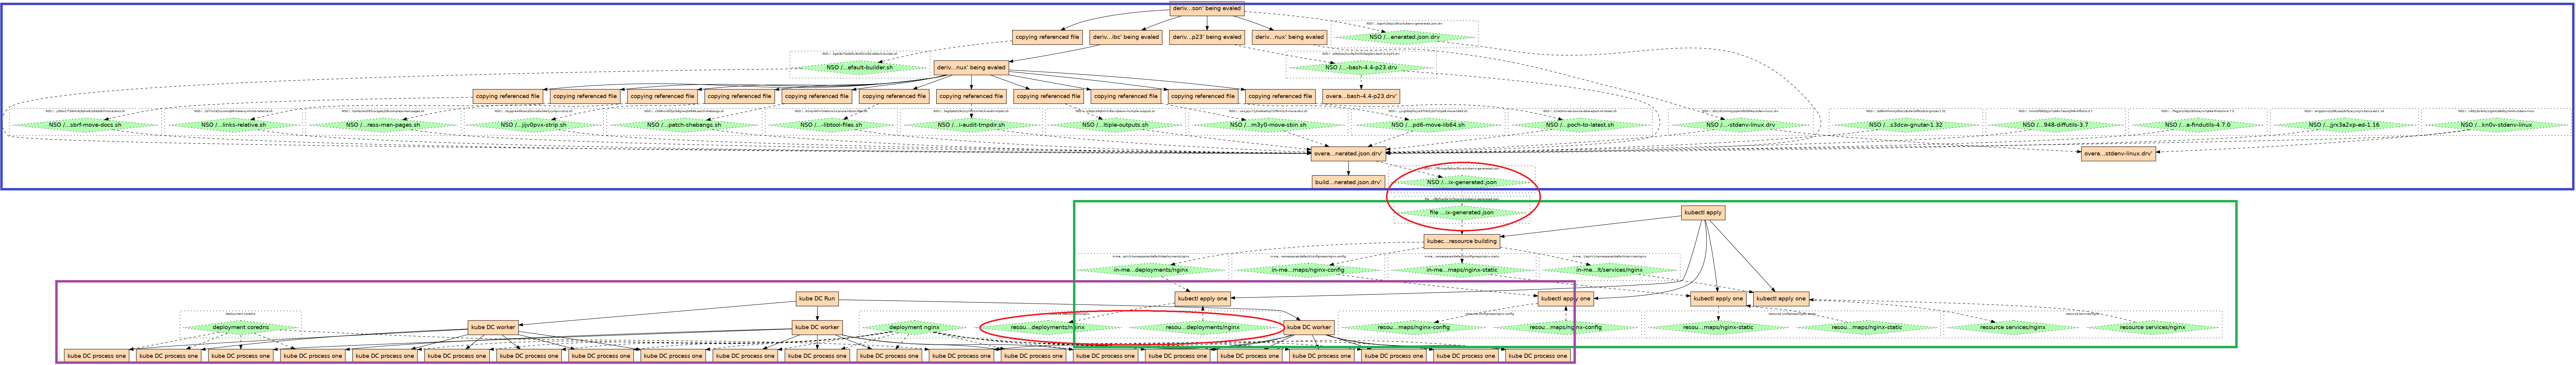
\includegraphics[scale=0.1]{img/huge-graph-3.png}
    \end{sideways}
    \vspace{-1em} 
    \caption{Extract from Tenmo record of a HCPS composed out of Nix / KubeNix, kubectl, and Kubernetes deployment controller.} 
    \label{fig:huge-graph-dot}
\end{figure}

\Cref{fig:huge-graph-dot} represents a Hierarchical Control Plane System composed out of these components and tracked by Tenmo. The top part outlined with indigo color rectangle is an extract from the KubeNix build process for a deployment. The right part outline in light green color is an extract of a record of Kubectl execution (as described in \cref{fig:kubectl}. The bottom part is an extract of a Kubernetes deployments controller performing an intent-based actuation of a deployment resource (as described in \cref{sec:k8s-depl-controller}). Full Tenmo traces would not be possible to visualize in a thesis using existing Graphviz-based tooling.

The Kubnix build and Kubectl execution are related via the file \texttt{kubenix-generated.json} built by Kubenix and consumed by Kubectl. Kubectl and Kuberentes deployments controller are linked via the deployment resource representation submitted to Kubernetes by Kubectl tool. These are marked in red circles in \cref{fig:huge-graph-dot}.

This shows that Tenmo is able to track activity and trace provenance of objects across multiple levels of a hierarchical system. Although this is a simplified example, covers the peculiarities of HCPS systems described in \fullref{sec:intro}.






\begin{comment}

\section{Solution scalability}
%% GP: Czy możemy to w ogóle wywalić? To miało omawiać na ile rozwiązanie się skaluje z kodem, z ludźmi, z systemem, etc?

\subsection{Performance}
%% GP: Czy możemy to pominąć? Wyniki nie będą oszałamiające, a czasu już nie ma.

Rudimentary performance testing has been performed of Nix builds with and without producing JSON logs.

\begin{itemize}
	\item As an extra sanity check, basic performance numbers, not a proper benchmark, maybe show trend with 2x more data.
    \begin{itemize}
    	\item E.g. k8s deployment at size X and 10X, requests still are fast enough
    \end{itemize}
\end{itemize}

TODO: Time to process as events per seconds.


\end{comment}




\begin{comment}
NOTATKI:
\begin{itemize}
\item Uzasadnić dlaczego narzędzie się skaluje lepiej, niż człowiek
\item Skalowanie z linijkami kodu, modułów, zespołów, równolegle wystawianych do produkcji, etc.
\item Wspomnieć o gitops, scaling with repo size, scaling with infrastructure as code, etc.
\end{itemize}
\end{comment}
